\documentclass[a4paper, 10pt]{article}
\usepackage{graphicx}
\usepackage{amsmath}
\usepackage{hyperref}
\hypersetup{colorlinks=false}

\author{George Zakhour}
\title{{\bf Simulating a two dimensional particle in a square quantum box with
        CUDA}}
\date{\today}

\begin{document}

\maketitle
\newpage
\tableofcontents
\newpage

\section{Background, Motive and Experiment}
The particle in box problem is one of the first problems given to undergraduate
students in a course about quantum mechanics. It showcases how the energy
of particles is quantized and it highlights the probabilistic nature of
quantum mechanics, especially with the idea that the particle is not located in
a fixed position but it has a likelihood of existing at any point in space.\\\\
The particle in a box is an experiment in which a particle is stuck inside a
box and cannot escape. The energy outside this box is $\infty$ while inside it
is $0$. The particle thus moves inside the box of dimensions $L$x$L$.\\\\
Trying to imagine how these probabilities are scattered in the box is hard and one
can't do without a simulation of the physical properties of the particle
(position, energy and momentum).\\\\
In this simulation I try and simulate the "particle in a box" problem to
display the probabilities of the position and the energy of the particle at
each state.

\section{Expected Output}
Searching online, I have found a Youtube video that simulates the particle in a
box\footnote{ Particle in a Box - Youtube {\emph
http://www.youtube.com/watch?v=jevKmFfcaxE}}, but lacks essential information
on the state of the system, for example the dimensions of the box and the
energy levels of the particle at each frame. Although lacking these
essential variables I will base my results on the video.\\

\begin{figure}[hb]
    \centering
        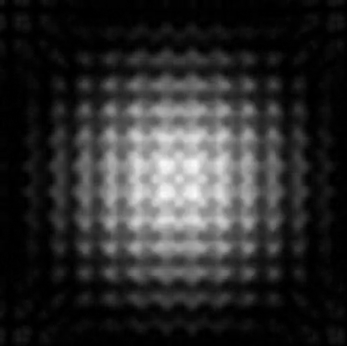
\includegraphics[width=5cm]{graphics/online_simulation.png}
    \caption{A screenshot of a "particle in a box" simulation found on Youtube}
\end{figure}

\newpage

\section{The mathematics of a particle in a box}
    \subsection{In one dimension}
        \subsubsection{Finding the Wave Function from Schrodinger's Equation}
        \label{sec:wave_equation_oned}
        The time dependent Schrodinger equation is given as:
        \begin{equation} \label{eq:time_dependant_equation}
            \left ( \frac{-\hbar^2}{2m} \nabla^2 + V \right ) \Psi(x,t)
            = i\hbar\frac{\partial}{\partial t}\Psi(x, t)   
        \end{equation}
        The time independent Schrodinger equation is given as:
        \begin{equation} \label{eq:time_independent_equation}
            \left ( \frac{-\hbar^2}{2m} \nabla^2 + V \right ) \Phi(x)
            = E \Phi(x)
        \end{equation}
        Where $\Psi$ is the wave equation. In terms of $\Phi$, $\Psi$ is
        denoted as:
        \begin{equation} \label{eq:dep_in_equation}
            \Psi(x, t) = e^{-i(E/\hbar)t}\Phi(x)
        \end{equation}
        Assuming the following is a solution to (\ref{eq:time_independent_equation}):
        \begin{equation} \label{eq:assumed_solution}
            \Phi(x) = A\cos(kx) + B\sin(kx)
        \end{equation}
        And given these two conditions that arise from the experiment:
        $$ \Phi(0) = \Phi(L) = 0 $$
        We plug them in the (\ref{eq:assumed_solution}) and find the following:
        \begin{align}
            \left\{\begin{matrix}
            A & = & 0 \\ 
            k & = & \frac{n}{L}\pi & \text{(n is the energy level)}
            \end{matrix}\right.
        \end{align}
        To find the value of $B$ we need to normalize the equation.\\
        The probability of finding the particle inside $[0; L]$ is $1$ because
        it cannot escape.
        \begin{align}
            \int_{0}^{L} |\Phi|^2 dx &= 1  \\
            B^2\int_{0}^{L} \sin^2\left ( \frac{n}{L}\pi x \right ) dx &= 1
        \end{align}
        And thus $B = \sqrt{\frac{2}{L}}$.\\
        Finally we get the solution to the time independent Schrodinger equation
        \begin{align}
            \Phi(x) = \sqrt{\frac{2}{L}}\sin(\frac{n}{L}\pi x)
        \end{align}

        \subsubsection{Energy at each quantum level $n$}
        \label{sec:energy_oned}
        We note the following
        \begin{align}
            \frac{\partial^2 }{\partial x^2} \Phi = -\left (
            \frac{n\pi}{L}\right )^2 \Phi
        \end{align}
        If we replace the results in (\ref{eq:time_independent_equation}) we find:
        $$ E_n = \frac{\hbar^2 n^2 \pi^2}{ 2 m L^2} $$
        Or simply:
        \begin{align*}
            E_n &= n^2 E_1 \\
            E_1 &= \frac{\hbar^2 \pi^2}{2 m L^2}
        \end{align*}

        \subsubsection{Probability function of the position}
        \label{sec:position_oned}
        The probability of finding the particle between $a$ and $b$ is the following:
        \begin{equation} \label{eq:probability_position}
            \left\{\begin{matrix}
            \int_{a}^{b} |\Phi|^2 dx & \text{if} \; \: a,b \in [0, L] \\ 
            0 & \text{otherwise}
            \end{matrix}\right.
        \end{equation}
        If we wish to find the position inside a box of width $\epsilon$ and
        center $a$ we would integrate between $a-\epsilon/2$ and $a+\epsilon/2$
        where both ends are between $0$ and $L$\\
        The integration will lead to the following:
        $$ P(x) = \frac{\epsilon}{L} + \frac{1}{2n\pi} \left [ 
            \sin\left ( \frac{2n\pi}{L}(a - \epsilon/2)\right ) -
            \sin\left ( \frac{2n\pi}{L}(a + \epsilon/2)\right )
        \right ]$$
        Which can be reduced more to the following form:
        $$ P(x) = \frac{\epsilon}{L} - \frac{1}{n\pi}\sin\left( \frac{n\pi}{L}\epsilon \right)
        \cos\left(\frac{2n\pi}{L}x\right)$$

    \subsection{In two dimensions}
        \subsubsection{The time-independent solution}
        This time we suppose the solution is
        \begin{equation} \label{eq:suppose_twod_solution}
            \Phi(x, y) = X(x)Y(y)
        \end{equation}
        \begin{align*}
            X(x) &= A\cos(k_x x) + B \sin(k_x x) \\
            Y(y) &= C\cos(k_y y) + D \sin(k_y y) \\
        \end{align*}
        Plugging (\ref{eq:suppose_twod_solution}) in (\ref{eq:time_independent_equation})
        and doing similar operations as \emph{~\ref{sec:wave_equation_oned}} we get
        the following solution:
        \begin{equation} \label{eq:twod_solution}
            \Phi(x, y) = \frac{2}{L} \sin\left( \frac{n_x\pi}{L}x\right)
                         \sin\left( \frac{n_y\pi}{L} y\right)
        \end{equation}

        \subsubsection{Energy in two dimensions}
        Doing the same steps as \emph{~\ref{sec:energy_oned}} we find that the energy has
        become:
        \begin{align}
            E_{n_x, n_y} &= \frac{\hbar^2 \pi^2}{2mL^2} (n^2_x + n^2_y)
        \end{align}
        Or simply:
        \begin{align*}
        E_{n_x, n_y} &= (n^2_x + n^2_y) \; E_{1,1} \\
        E_{1,1} &= \frac{\hbar^2 \pi^2}{2mL^2} 
        \end{align*}

        \subsubsection{Probability function of the position}
        Similar to section \emph{~\ref{sec:position_oned}} to find the
        probability of finding the particle inside the box of size
        $\epsilon$x$\epsilon$ we integrate the wave function inside a
        box of center $(x,y)$ and width $\epsilon$.
        $$ P(x, y) = \int^{y+\epsilon/2}_{y-\epsilon/2}\int^{x+\epsilon/2}_{x-\epsilon/2}
          |\Phi(x, y)|^2 dx dy $$
        After evaluating the integral we get the following function:
        \begin{equation} \label{eq:position_twod_equation}
            P(x, y) = \frac{1}{L^2} \; p(x) \; p(y)
        \end{equation}
        $$
        p(\alpha) = \epsilon - \frac{L}{n_\alpha\pi} \cos\left( \frac{2n_\alpha\pi}{L}\alpha \right)
        \sin\left( \frac{n_\alpha\pi}{L} \epsilon\right)
        $$

        \subsection{Generalizing the time-independent solution}
        The equation that we have found so far depends on two quantum numbers
        $n_x$ and $n_y$ and describes the particle for these energy levels only.
        However the final time-dependant equation is a combination of many of these
        equations. The final time-independent equation is:
        \begin{equation} \label{eq:general_position}
            \Phi(x,y) = \sum_{n} c_n \Phi_{n_x, n_y}(x,y)
        \end{equation}
        Where the constant $c_n$ is the square root of the probability of getting
        the equation $\Phi_{n_x, n_y}$ that describes the particle in the box.

        \subsection{Generalizing the probability function}
        Since we have a more general wave function we need to have a more general
        probability function for the position. The new definition is generated from
        integrating $\Phi$ between $a-\epsilon/2$ and $a+\epsilon/2$. The result is:
        $$ P(x, y) = \sum_{n} c^2_n \: P_n(x, y)$$

\newpage

\section{Implementation}
    \subsection{Synopsis}
    This simulation will display the probability of finding the particle in sub-boxes in the box
    as well as display the energy in the sub-box of width $\epsilon$. Each frame displays the
    particle with a new set of probabilities for each energy level.\\\\
    The probability of the position will be visualized by the intensity of the color. The brighter
    the color, the higher the probability.\\\\
    The energy however will be visualized using the standard colors assigned to energies; lower
    energies have blue-shades while high energies have red-shades.

    \subsection{Conventions}
    Some of the conventions adopted throughout the code are
    \begin{itemize}
        \item words in functions, structs and variable names are separated by an \_ (underscore)
        \item CUDA kernels start with the keyword \texttt{cuda\_}.\\
              For example \texttt{cuda\_probability}
        \item CUDA device functions start with \texttt{cuda\_} and end with \texttt{\_device}.\\
              For example \texttt{cuda\_probability\_1d\_device}
        \item Tiny mathematical and physical constants, such as $\hbar$ are expressed
              as float numbers without their orders.\\ For example $\hbar = 1.054\cdot10^{-34}$
              is defined as \texttt{\#define HBAR 1.054}
    \end{itemize}

    \subsection{Brightness and Color mapping}
        \subsubsection{Brightness}
        The intensity of the colors denote the probability of finding the particle. Since
        probabilities are always between 0 and 1, converting them to intensities is just
        a matter of mapping the probabilities from $[0, 1]$ to $[0, 255]$.\\\\
        However $\epsilon$ is a small number, so the probability is always small; usually
        less than $0.1\%$. Therefore we need to find the highest probability in the space
        and remap from $[0, \text{max}]$ to $[0, 255]$. At first I have tried to brute force
        the problem exploiting my GPU using functions to find maximums using reduction. But
        the process of finding the highest probability of a particle with 10 energy levels
        inside a box divided into 262,144 boxes took around 28ms. Allowing me to get only
        35fps in the animation.\\
        A new solution needed to be adopted and I went over the equations again to try and
        find that maximum analytically. My results are:\\\\
        For $p(\alpha)$ to be maximal
        $$\frac{\epsilon}{L} - \frac{1}{n_{\alpha}\pi} \sin\left(\frac{n_{\alpha}\pi}{L}\epsilon\right)
        \cos\left(2\frac{n_{\alpha}\pi}{L}\alpha\right)$$
        needs to be maximal.  And this is achieved when $\cos{x} = -1$ which is possible
        since $0 \leq x \leq 2\pi$. Therefore the highest probability for one energy
        level is: 
        $$\frac{\epsilon}{L} + \frac{1}{n_{\alpha}\pi} \sin(\frac{n_{\alpha}\pi}{L}\epsilon)$$
        Following similar analysis we can deduce that the highest probability (denoted by
        $m$) is close to,
        but not exactly:
        $$m = m_x . m_y$$
        $$m_{\alpha} = \frac{\epsilon}{L} + \sum_i \left ( c^2_i \frac{1}{n_{\alpha_i}\pi}
        \sin\left(\frac{n_{\alpha_i}\pi}{L}\epsilon\right) \right )$$\\\\
        \textbf{UPDATE} After implementing and testing the algorithm the uncertainty in the algorithm
        has proved to be overwhelming and the probabilities' range was no longer $[0, 1]$ but much smaller.
        Therefore a fallback was needed.\\\\
        The approach followed was a bruteforce solution where we compute the probabilities at each at each
        pixel and search for the largest. However to make the searching faster a reduction algorithm
        was adopted to speed it up. The algorithm creates a much smaller array in which it stores
        the maximum of a chunk of the original array. Then on the CPU we loop over the results (which are
        usually 32) and pick the maximum of these. The following illustration describes how the maximum
        reduction algorithm works
        \begin{figure}[hb]
            \centering
                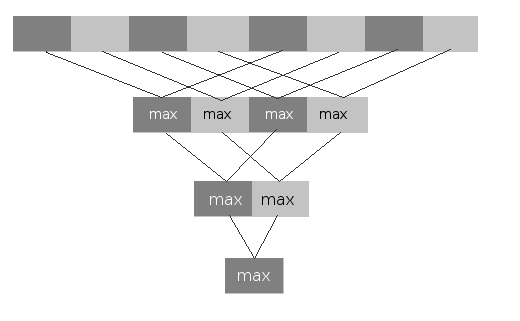
\includegraphics[width=8cm]{graphics/max_reduction.png}
            \caption{Finding the maximum element in an array using reduction}
        \end{figure}
        The fact that this algorithm was used adds a restriction on the dimensions of the window. The height
        and the width of the window need to be a power of 2 for this algorithm to work effectively.
        No solution has been made up yet to generalize the dimensions of the window.
        
        \subsubsection{Tint and Color}
        The tint in the color represents the energy of the particle. Red is the highest
        energy and blue is the lowest. If we can map the energy in an interval between
        0 and 1 we can easily get the RGB values. The following equation can be applied
        $$ \begin{bmatrix} R_{xy} \\ G_{xy} \\ B_{xy} \end{bmatrix} = P(x, y)
        \begin{bmatrix} 255E \\ 20 \\ 255(1-E) \end{bmatrix} $$
        Where $P(x, y)$ is the probability of finding the particle at $(x, y)$ and between
        0 and 1. And $E$ is the energy remapped between 0 and 1. \\\\
        To problem of remapping the energy is easy to solve. Through mathematical analysis
        we can show that the highest energy we can find is
        $$ E_{max} = (n^2_{max_x} + n^2_{max_y})\frac{\hbar^2\pi^2}{2mL^2} $$
        And therefore we can remap any energy we find to a value in the interval $[0, 1]$
        and find the corresponding RGB values.

        \subsection{Next set of probabilities}
        Every frame in the animation consists of a new set of probabilities close to the ones of the
        previous frame. A problem came up and that is how to generate new set of probabilities close
        to the ones in the previous frame to insure the smooth animation between the frames.\\\\
        The model adopted to insure the smoothness and the continuity in the probabilities consists
        of multiple sine waves where the period of one is 10 times more than its neighbor and so on.
        If plotted, the model looks like the following: (the sines were stretched vertically for a better
        visualization)
        \begin{figure}[hb]
            \centering
                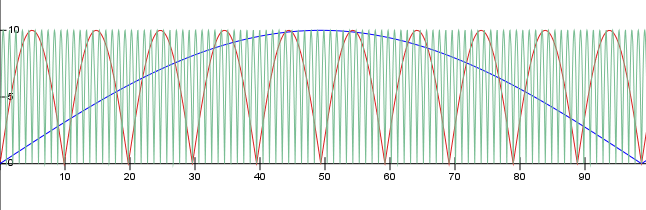
\includegraphics[width=8cm]{graphics/sine_probabilities.png}
            \caption{Plotting
               $x(t) = 10\left| sin \left( \frac{0.1}{\pi}t \right) \right|$, 
               $y(t) = 10\left| sin \left( \frac{1}{\pi}t \right) \right|$, 
               $z(t) = 10\left| sin \left( \frac{10}{\pi}t \right) \right|$}
        \end{figure}
        After finding the values of each sine wave at a time $t$ we can normalize the answers so that
        their sum is $1$. Bellow is a table representing some values normalized.
        \begin{center}
            \begin{tabular}{| c | c | c | c |}
                \hline
                \textbf{Time} & \textbf{x} & \textbf{y} & \textbf{z} \\ \hline
                0.1 & 0.0091 & 0.0915 & 0.8994 \\
                0.2 & 0.0096 & 0.0957 & 0.8947 \\
                0.3 & 0.0104 & 0.1035 & 0.8861 \\
                0.4 & 0.0116 & 0.1159 & 0.8725 \\
                0.5 & 0.0136 & 0.1350 & 0.8515 \\
                0.6 & 0.0166 & 0.1648 & 0.8186 \\
                0.7 & 0.0215 & 0.2135 & 0.7649 \\
                0.8 & 0.0304 & 0.3006 & 0.6690 \\
                0.9 & 0.0490 & 0.4834 & 0.4675 \\
                1.0 & 0.0824 & 0.8102 & 0.1074 \\
                1.1 & 0.0479 & 0.4698 & 0.4822 \\
                1.2 & 0.0368 & 0.3590 & 0.6042 \\
                1.3 & 0.0322 & 0.3134 & 0.6544 \\
                1.4 & 0.0309 & 0.2987 & 0.6704 \\
                1.5 & 0.0317 & 0.3053 & 0.6630 \\
                1.6 & 0.0347 & 0.3324 & 0.6329 \\
                1.7 & 0.0405 & 0.3859 & 0.5736 \\
                1.8 & 0.0509 & 0.4818 & 0.4673 \\
                1.9 & 0.0701 & 0.6595 & 0.2704 \\
                2.0 & 0.0859 & 0.8022 & 0.1119 \\ \hline
            \end{tabular}
        \end{center}
        \begin{center}Table 1: Values from $x(t)$, $y(t)$ and $z(t)$ at different times\end{center}
        A general formula can be deduced to find the equation of the nth wave.
        \begin{align}
            P_{n}(t) = \left| sin\left( \frac{10^{1-n}}{\pi}t \right)\right|
        \end{align}

\newpage
\section{API}

\newpage
\section{Results}

\newpage
\section{Code License: GNU General Public License}
Copyright (C) 2013 George Zakhour\\

This program is free software: you can redistribute it and/or modify it under
the terms of the GNU General Public License as published by the Free Software
Foundation, either version 3 of the License, or (at your option) any later
version.\\

This program is distributed in the hope that it will be useful, but WITHOUT ANY
WARRANTY; without even the implied warranty of MERCHANTABILITY or FITNESS FOR A
PARTICULAR PURPOSE. See the GNU General Public License for more details.\\

You should have received a copy of the GNU General Public License along with
this program. If not, see http://www.gnu.org/licenses/.\\


\end{document}
